\documentclass[]{article}
\usepackage{amsmath}
\usepackage{graphicx} % to insert pictures
\usepackage{listings}
\usepackage{color}

\definecolor{dkgreen}{rgb}{0,0.6,0}
\definecolor{gray}{rgb}{0.5,0.5,0.5}
\definecolor{mauve}{rgb}{0.58,0,0.82}

\lstset{frame=tb,
	language=R,
	aboveskip=3mm,
	belowskip=3mm,
	showstringspaces=false,
	columns=flexible,
	basicstyle={\small\ttfamily},
	numbers=none,
	numberstyle=\tiny\color{gray},
	keywordstyle=\color{blue},
	commentstyle=\color{dkgreen},
	stringstyle=\color{mauve},
	breaklines=true,
	breakatwhitespace=true,
	tabsize=3
}



\title{LASSO and sub-sampling}

\begin{document}
\maketitle

\section{Review of LASSO}
The LASSO is essentially an optimization problem with constraint on L1-norm of parameters, which is a typical quadratic programming problem.


\begin{align}
	\hat{\beta}^{lasso} & = \underset{\beta}{\arg\max} \sum_{i=1}^{N}(y_i-\beta_0-\sum_{j=1}^{p}x_{ij}\beta_j)^2\\
	&\text{subject to}
	\sum_{j=1}^{p}|\beta_j|\leq t \notag
\end{align}
Here, t is the tuning parameter, which is usually selected by cross-validation.\\
\\
If we assume there are only 2 parameters to optimize, the RSS has elliptical contours centered at the OLS estimate. The constraint $|\beta_1|+|\beta_2| \leq t$ is just a diamond region. The LASSO method is to find the first point where the elliptical contours hit the constraint region. Since the constraint region has sharp corners on axis, the solution will usually occur on the axis, then it has one parameter $\beta_j = 0$ This is why LASSO good for variable selection, i.e. “p reduction”. The following figure well illustrates this.\\
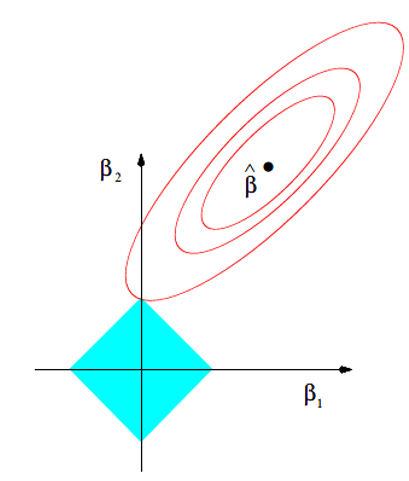
\includegraphics[width = .7\textwidth]{l1_select.png}\\
Equivalently, we can reparametrize the problem in the form of “squared-error loss + L1-penalty”, i.e. the Lagrangian form:
\begin{equation}
	\hat{\beta}^{lasso} = \underset{\beta}{\arg\max}\{   \frac{1}{2}\sum_{i=1}^{N}(y_i-\beta_0-\sum_{j=1}^{p}x_{ij}\beta_j)^2 + \lambda\sum_{j=1}^{p}|\beta_j|\}
\end{equation}
The $\lambda$ is the tuning parameter, which has 1-to-1 correspondence to t. The $L_1$-penalty makes the solutions nonlinear in the $y_i$, so there’s no closed form for solutions.\\
\\
To get the solution, one naive way is to view the LASSO problem in a Bayesian way, and use MCMC to get the estimate. If we set the prior for each parameter as double exponential (Laplace) distribution, with pdf be $\frac{1}{2\tau}exp(-\frac{|\beta|}{\tau})$ and $\tau=\frac{1}{\lambda}$, then the function in curly bracket of equation (2) is just the negative log-posterior density of $\beta$, and the LASSO estimate is the mode of the posterior distribution. However, this method is very inefficient.\\
\\
Least angle regression (LAR) provide an efficient way to compute the entire LASSO path. The idea of LAR is similar to forward stepwise selection but do it in a “smooth and less greedy “way. (Another idea is to do a stagewise, i.e. “boosting”, version, but this is less efficient than LAR). Roughly speaking, at first step LAR selects the variable most correlated with the response and move toward its least square value. When there’s another variable share the same correlation with residuals, the process is paused. The second variable joins and move together in a way that keeps correlations tied and decreasing. Keep this process until all variables are in the model. This process is perfectly illustrated in the following plot:\\
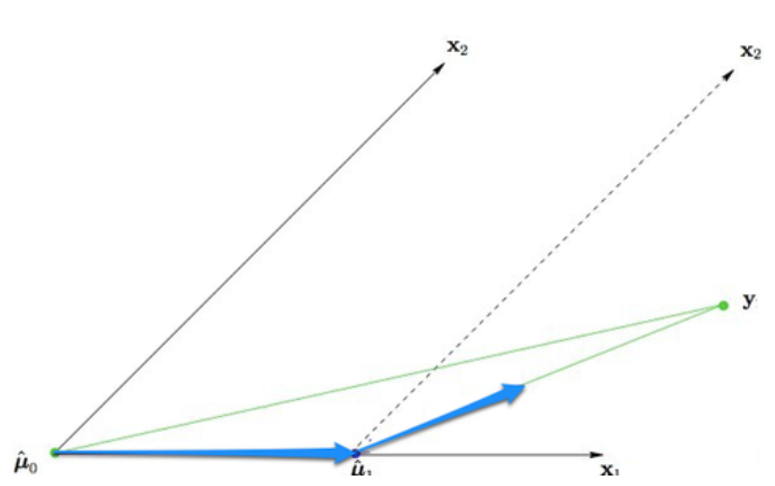
\includegraphics[width = .7\textwidth]{LAR.png}\\
\\
To give LASSO path, we only need to add one more criterion. If a non-zero coefficient hits 0, drop this variable from the “active set” of variables and recompute the current joint least squares direction.\\
\\
Another approach to solve LASSO problem is the coordinate descent. The idea is to fix the $\lambda$ and
optimize successively over each parameter, holding the other parameters fixed at their current values. The process keeps going until convergence. Denote current estimate for $\beta_k$ as $\tilde{\beta}_k(\lambda)$ , we can rearrange as follows to isolate $\beta_j$:
\begin{equation}
	R(\tilde{\beta}(\lambda), \beta_j) =   \frac{1}{2}\sum_{i=1}^{N}(y_i-\sum_{k \ne j}x_{ik}\tilde{\beta}_k(\lambda) - x_{ij}\beta_j)^2 + \lambda\sum_{k \ne j}|\tilde{\beta}_k(\lambda)| + \lambda |\beta_j|
\end{equation}
Then the problem reduce to a univariate LASSO problem and the resulting update is:
\begin{align}
	\tilde{\beta}_k(\lambda) &\gets S(\sum_{i=1}^{N}x_{ij}(y_i- \tilde{y}_i^{(j)}), \lambda)\\
	&\text{where } 
	S(t, \lambda)=sign(t)(|t|-\lambda)_{+} \text{is the soft-thresholding opertor} \notag
\end{align}
The coordinate descent can be used to compute solutions at a grid of $\lambda$. Basically, we can search $\lambda$ from above, and use the estimates from previous step as a “warm start”. In large problems, coordinate descent can be faster than LARS.\\
\\
One drawback for LASSO regression is not asymptotic consistent: it may cause the estimates of the non-zero coefficients to be 0. One way is to modify the LASSO penalty so that larger coefficients are shrunken less severely. SCAD penalty uses this idea: it replaces $\lambda |\beta|$ by $J_a (\beta, \lambda)$, where
\begin{equation}
	\frac{dJ_a(\beta, \lambda)}{d\beta}=\lambda\cdot sign(\beta)[ \,I(|\beta|\leq\lambda) + \frac{(a\lambda-|\beta|)_{+}}{(a-1)\lambda}I(|\beta| > \lambda)] \,
\end{equation}
for some $a\geq 2$. However, SCAD is not convex. The adaptive LASSO solves this problem: it is both consistent and convex. Adaptive LASSO uses a weighted penalty of the form $\sum_{j=1}^{p}w_j|\beta_j|$ where $w_j=1/|\hat{\beta}_j|^{\nu}$, $\hat{\beta}_j$ is the OLS or ridge estimate.\\
\\
\section{A Rough Idea of Combining Sub-sampling and Adaptive LASSO}
Here I’m thinking to use adaptive LASSO to achieve asymptotic consistency. The main goal is to get the optimized subsampling probability (SSP) for the full data: assign larger probabilities to observations with more information.\\
\\
To do that, we may follow the rationale of OSMAC, i.e. find the asymptotic distribution of $\hat{\beta}_{A-lasso}^{S}-\hat{\beta}_{A-lasso}^{F}$, where $\hat{\beta}_{A-lasso}^{S}$ is the adaptive LASSO solution under subsamples and $\hat{\beta}_{A-lasso}^{F}$ is the adaptive LASSO solution under full data. Then we can derive SSP by minimizing the trace of asymptotic variance (A-optimization) or doing L-optimization. But I don’t know if it is possible.\\
\\
My intuition is that maybe we can treat the adaptive LASSO solution as MLE and implement SSC derived before, since adaptive LASSO has the "oracle property". Well, it should be incorrect...
But I still tried to run simulations to see what will happen.\\
\\
The data is generated follow as mzNormal, but the dimension of $\beta$ is 40, with the first 10 to be 0.5 and the remaining 30 be 0. The data is generated as follows:\\
\begin{lstlisting}
set.seed(123)
n <- 10000
nBeta <- 40
beta <- rep(0, nBeta)
beta[1:10] <- 0.5
Sigma <- matrix(0.5, nrow = nBeta, ncol = nBeta)
diag(Sigma) <- 1
mu <- rep(0, nBeta)
X <- mvrnorm(n, mu, Sigma)
eta <- X %*% beta
p <- exp(eta)/(1 + exp(eta))
y <- rbinom(n, 1, prob = p)
\end{lstlisting}

Then I basically did something as unweighted OSMAC, based on subsampling with replacement. The pilot and second step estimates have not combined yet. The uniform subsampling is shown for reference. Here, I only tried adaptive LASSO version of mMSE and mVc, since glm for small observations (subsamples) will not converge in this case.\\
\\
For example, this is the mVc for adaptive LASSO:\\
\begin{lstlisting}
	mVC.mse.adlasso <- rep(NA, length(r))
	mVC.mse.true <- rep(NA, length(r))
	mVC.mse.mle <- rep(NA, length(r))
	for(i in 1:length(r)){
		mVC.beta.boot <- matrix(NA, nrow = S, ncol = nBeta)
		for(j in 1:S){
			n1 <- sum(y)
			n0 <- n - n1
			pilot.ssp <- rep(1/(2*n0), n)
			pilot.ssp[y==1] <- 1/(2*n1)
			pilot.idx <- sample(1:n, r0, replace = T, prob = pilot.ssp)
			pilot.y <- y[pilot.idx]
			pilot.X <- X[pilot.idx, ]
			pilot.beta <- adapt.lasso(pilot.X, pilot.y)
			pilot.eta <- X %*% pilot.beta
			pilot.prob <- exp(pilot.eta)/(1 + exp(pilot.eta))
			
			mVC.ssp <- abs(y - pilot.prob)*sqrt(apply(X^2, 1, sum))
			mVC.ssp <- mVC.ssp/sum(mVC.ssp)
			mVC.idx <- sample(1:n, r[i], replace = T, prob = mVC.ssp)
			mVC.y <- y[mVC.idx]
			mVC.X <- X[mVC.idx, ]
			mVC.beta <- adapt.lasso(mVC.X, mVC.y)
			mVC.beta.boot[j, ] <- mVC.beta + pilot.beta
		}
		
		mVC.mse.adlasso[i] <- mean(apply((mVC.beta.boot -
		matrix(rep(beta.adpLasso, S),nrow = S, byrow = T))^2,
		1, sum))
		mVC.mse.true[i] <- mean(apply((mVC.beta.boot -
		matrix(rep(beta, S),nrow = S, byrow = T))^2,
		1, sum))
		mVC.mse.mle[i] <- mean(apply((mVC.beta.boot -
		matrix(rep(beta.mle, S),nrow = S, byrow = T))^2,
		1, sum))
	}
\end{lstlisting}
Here, \textbf{three versions of MSE are calculated}: (1) $MSE_{A-LASSO}=S^{-1}\sum_{s=1}^{S}|| \breve{\beta}^{(s)} - \hat{\beta}_{A-LASSO}||^2$, (2) $MSE_{MLE}=S^{-1}\sum_{s=1}^{S}|| \breve{\beta}^{(s)} - \hat{\beta}_{MLE}||^2$ and (3) $MSE_{true}=S^{-1}\sum_{s=1}^{S}|| \breve{\beta}^{(s)} - \beta_{true}||^2$. Here, $\breve{\beta}^{(s)}$ is the estimate from the $s^th$ subsample, $\hat{\beta}_{A-LASSO}$ is Adaptive LASSO estimate from full data, $\hat{\beta}_{MLE}$ is the MLE estimate from full data and $\beta_{true}$ is the true value.\\
\\
The results are as follows:\\
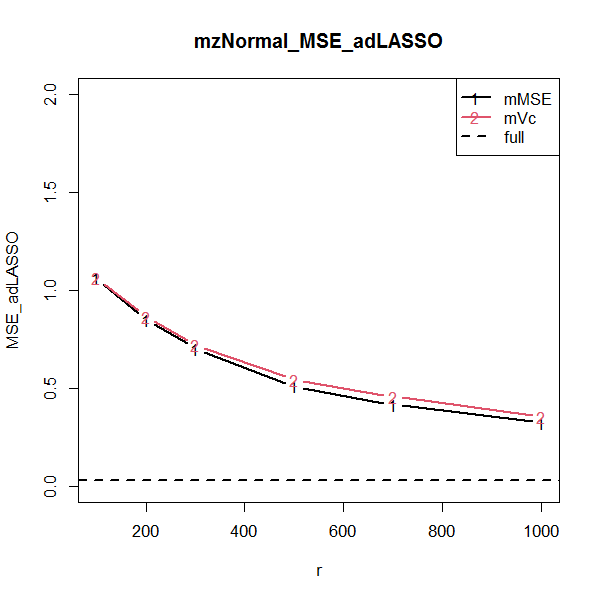
\includegraphics[width = .5\textwidth]{MSE_adLASSO.png}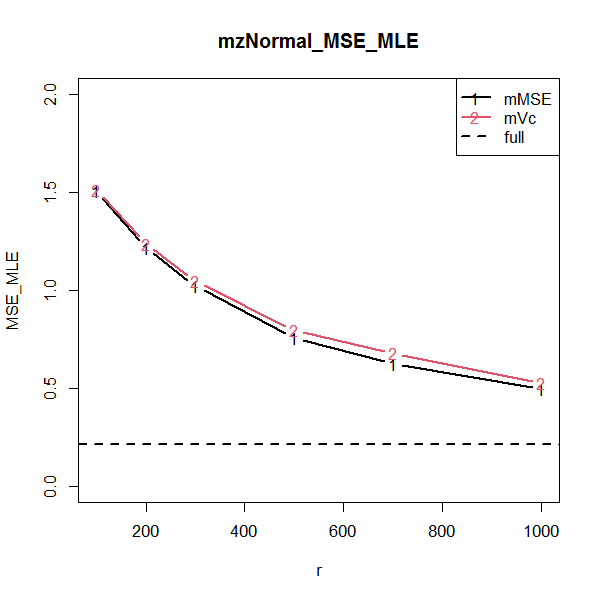
\includegraphics[width = .5\textwidth]{MSE_MLE.png}
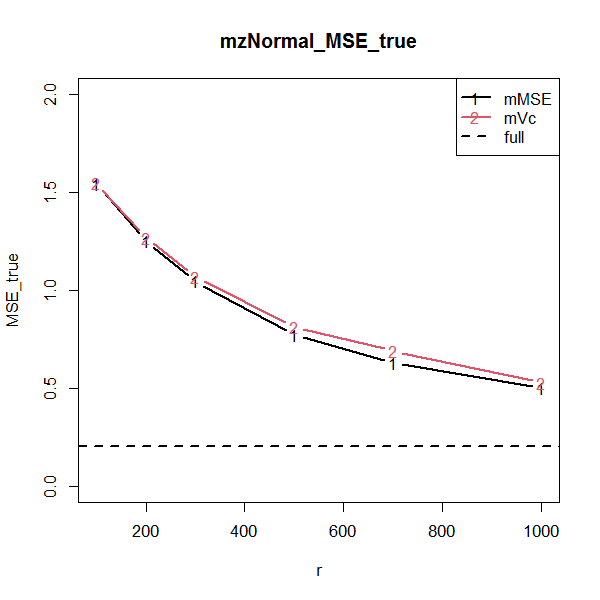
\includegraphics[width = .5\textwidth]{MSE_true.png}\\
I'm not sure if this make sense...


\end{document}
